Para reduzir significativamente a dimensão dos mapas de características, eventualmente, após a camada convolucional, é utilizada uma camada chamada \textit{pooling}. A camada de \textit{pooling} divide o mapa de características de entrada em blocos de tamanhos iguais e processa cada bloco para criar um mapa de características condensado. O processamento dos blocos é definido por uma função de \textit{pool} que pode ser, por exemplo, a função máxima. Assim como na camada de convolução, na camada de \textit{pooling} também é preciso especificar o tamanho da região de \textit{pooling} e o \textit{stride} $s$ da operação, conforme exemplificado na Figura \ref{img:pooling} em que a região possui tamanho 2 x 2 e o \textit{stride} $s=1$ \cite{ref:buduma,ref:khan}.

\begin{figure}[!ht]
	\centering
	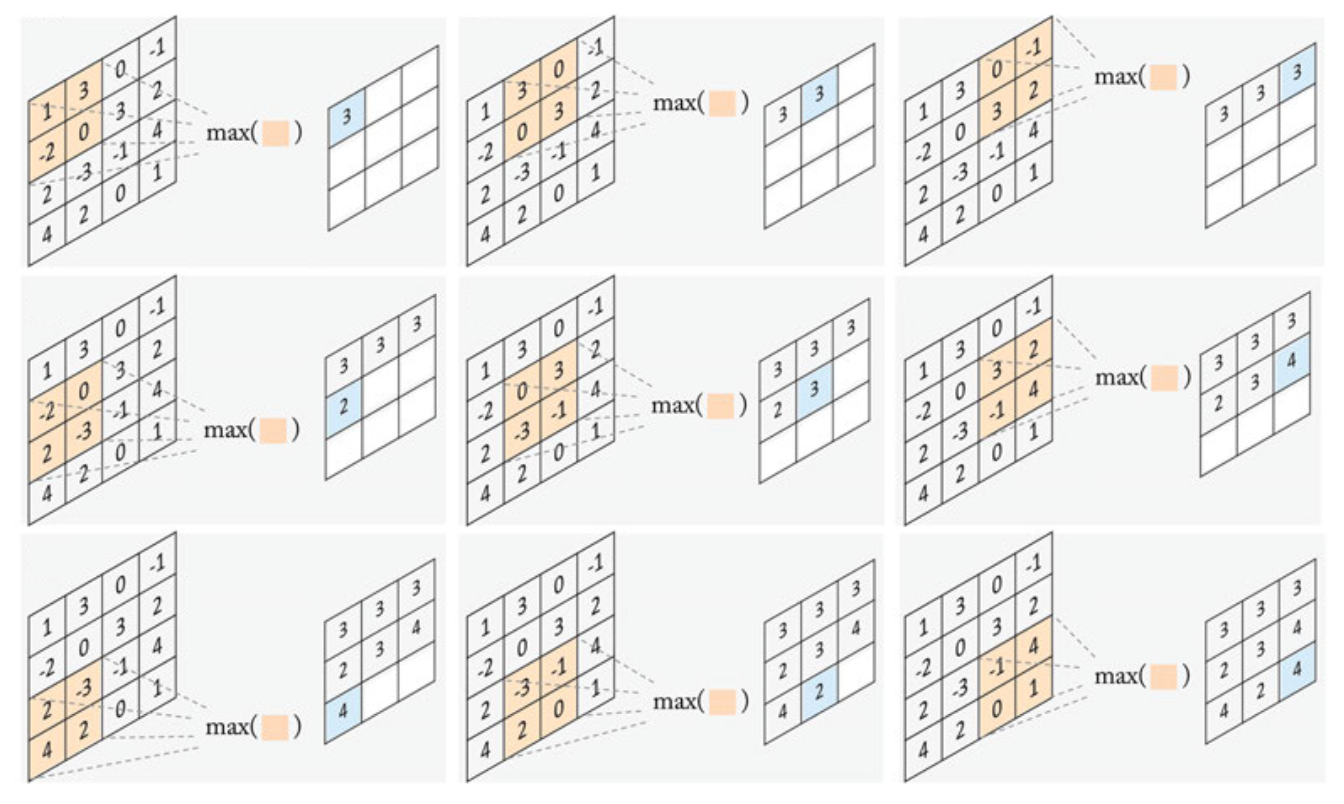
\includegraphics[width=0.9\textwidth]{./img/pooling}
	\caption{Exemplo de um processo de \textit{pooling} aplicado em uma entrada de tamanho 5 x 5 e uma região \textit{pooling} de tamanho 2 x 2. Fonte: \cite{ref:khan}.}
	\label{img:pooling}
\end{figure}